% -*- mode:flyspell; mode:latex -*-
\documentclass[12pt]{article}

% \addtolength{\oddsidemargin} {-0.885in}
% \addtolength{\textwidth}{1.75in}
% \addtolength{\evensidemargin}{-0.8in}
% topmargin -0.5in
\usepackage[a4paper, top=1cm, left=1.5cm, right=1.5cm]{geometry} % width= , 

\usepackage[latin1]{inputenc}
\usepackage[T1]{fontenc}
\usepackage[english]{babel}
\usepackage{graphicx}
\usepackage{float}


\usepackage{tikz}
\usepackage{[caption}
\usetikzlibrary{arrows}
\usetikzlibrary{decorations.markings}
\usetikzlibrary{decorations.pathmorphing}
% \usepackage[absolute,overlay]{textpos}
% \usepackage{onimage}

\usepackage{times}
\usepackage{graphics}

% \usepackage{subfigure}
% \usepackage{scalefnt}
%
% \renewcommand\thesubfigure{\arabic{subfigure}}

\usepackage{amsmath}
\usepackage{hyperref}
\usepackage{hhline}
\usepackage{subfig}
\usepackage{color}
\usepackage[all]{hypcap}

\usepackage[normalem]{ulem}  % for striking out
% \usepackage{fancyhdr}
% \pagestyle{fancy}
% \fancyhead[C]{}
% \fancyhead[L] {\it{Mu2e-doc-29670-v1.0} }
%%%%%%%%%%%%%%%%%%%%%%%%%%%%%%%%%%%%%%%%%%%%%%%%%%%%%%%%%%%%%%%%%%%%%%%%%%%%%%
% use natbib - biblatex not available on Mu2e interactive nodes
%%%%%%%%%%%%%%%%%%%%%%%%%%%%%%%%%%%%%%%%%%%%%%%%%%%%%%%%%%%%%%%%%%%%%%%%%%%%%%
\usepackage[square,sort,comma,numbers]{natbib}

% location of the .bib files: env var BIBINPUTS (~/library/bibliography)

% \usepackage[backend=biber, style=numeric-comp, sorting=ynt] {biblatex}
% \addbibresource{clfv.bib}

% \addbibresource{stntuple.bib}
% \addbibresource{mu2e_web.bib}
% \addbibresource{radiative_pion_capture.bib}

\graphicspath{{figures/}}
%%%%%%%%%%%%%%%%%%%%%%%%%%%%%%%%%%%%%%%%%%%%%%%%%%%%%%%%%%%%%%%%%%%%%%%%%%%%%%
% for portability, make sure all commands are included locally
% order them alphabetically
%%%%%%%%%%%%%%%%%%%%%%%%%%%%%%%%%%%%%%%%%%%%%%%%%%%%%%%%%%%%%%%%%%%%%%%%%%%%%%
% \include{commands}

\newcommand {\keVc}       {\mbox{$\rm keV\!/\!c$}}
\newcommand {\kmax}       {\mbox{$k_{\rm max}$}}

\newcommand {\MeVc}       {\mbox{$\rm MeV\!/c$}}
\newcommand {\MeVcsq}     {\mbox{$\rm MeV\!/c^2$}}

\newcommand {\mumemconv}[1][A] {\mbox{$\mu^- \textrm{#1} \rightarrow e^- \textrm{#1}$}}
% Define a relay to have 2 default arguments instead of limit of 1
\newcommand {\mumepconv}[1][A] {%
  \def\ArgI{{#1}}%store the first argument
  \mumepconvRelay
}
\newcommand \mumepconvRelay[1][A]  {\mbox{$\mu^- \textrm{\ArgI} \rightarrow e^+ \textrm{#1}$}}
\newcommand {\muminus}    {\mbox{$\mu^-$}}
\newcommand {\muplus}    {\mbox{$\mu^+$}}
\newcommand {\MuToEm}     {\mbox{$\mu^- \ra e^-$}}
\newcommand {\MuToEp}     {\mbox{$\mu^- \ra e^+$}}
\newcommand {\MuPToEp}    {\mbox{$\mu^+ \ra e^+$}}
\newcommand {\ra}        {\rightarrow}
\newcommand {\tandip}    {\mbox{$\tan \lambda$}}

\newcommand {\Pb}[1]     {\mbox{$\rm ^{#1}Pb$}}                 % isotopes of lead
\newcommand {\Au}[1]     {\mbox{$\rm ^{#1}Au$}}                 % isotopes of gold
\newcommand {\Ir}[1]     {\mbox{$\rm ^{#1}Ir$}}                 % isotopes of iridium
%%%%%%%%%%%%%%%%%%%%%%%%%%%%%%%%%%%%%%%%%%%%%%%%%%%%%%%%%%%%%%%%%%%%%%%%%%%%%%
% editing commands
%%%%%%%%%%%%%%%%%%%%%%%%%%%%%%%%%%%%%%%%%%%%%%%%%%%%%%%%%%%%%%%%%%%%%%%%%%%%%%
\newcommand {\add}[1]    {{\red #1}}
\newcommand {\alt}[1]    {{\green #1}} %alternate comment color
\newcommand {\del}[1]    {{\blue \sout{#1}}}
\newcommand {\dlt}[1]    {{\violet \sout{#1}}} %alternate delete color

\newcommand {\black}     {\color{black}}
\newcommand {\red}       {\color{red}}
\newcommand {\blue}      {\color{blue}}
\newcommand {\strike}[1] {{\blue \sout{#1}}}
%%%%%%%%%%%%%%%%%%%%%%%%%%%%%%%%%%%%%%%%%%%%%%%%%%%%%%%%%%%%%%%%%%%%%%%%%%%%%%
\begin{document}

\begin{titlepage}
  \begin{flushright}
    \bf {MU2E/PHYSICS/xxxxx} \\
    version 1.0
    \today
 \end{flushright}

  \vspace{1cm}

  \begin{center}
    {\Large \bf Commissioning of the Mu2e Data AcQuisition system and the Vertical Slice Test of the straw tracker

      \vspace{0.3in}

      11. Mu2e ROC simulation
    }

    \vspace{1cm}
    S. Gamba  \footnote{\texttt{Fermilab; e-mail:s.gamba2@studenti.unipi.it} (University of Pisa)
    P. Murat \footnote{\texttt{Fermilab; e-mail: murat@fnal.gov} (FNAL)

   
    version 1.0
    \today
 \end{flushright}

  \begin{abstract}
    This note presents an analysis of data coming from the teststand of the motherboard and the comparison with ROC simulation.
    \vspace{0.2in}
  \end{abstract}

\end{titlepage}
% \frontmatter
% \chapter*{Abstract}
%
% \addcontentsline{toc}{chapter}{Abstract}
%
% \mainmatter
%
{\tableofcontents}

%%%%%%%%%%%%%%%%%%%%%%%%%%%%%%%%%%%%%%%%%%%%%%%%%%%%%%%%%%%%%%%%%%%%%%%%%%%%%%%
%\chapter{Calibration}
%%%%%%%%%%%%%%%%%%%%%%%%%%%%%%%%%%%%%%%%%%%%%%%%%%%%%%%%%%%%%%%%%%%%%%%%%%%%%%%
% \input{input_data}

%%%%%%%%%%%%%%%%%%%%%%%%%%%%%%%%%%%%%%%%%%%%%%%%%%%%%%%%%%%%%%%%%%%%%%%%%%%%%%%
\newpage
\section {Notes for the authors}
\subsection {Revision history} 
\begin{itemize}
\item
  v1.01: initial version
\end{itemize}

%%%%%%%%%%%%%%%%%%%%%%%%%%%%%%%%%%%%%%%%%%%%%%%%%%%%%%%%%%%%%%%%%%%%%%%%%%%%%%
\section {Introduction}

In this note, we discuss several sources of beam-associated backgrounds,
not resulting from particle stops in the Mu2e stopping target. 
The backgrounds, which contributions are expected to be small,
could be split into three categories:

\begin{enumerate}
\item 
  $p_e > 100 \MeVc$ electrons scattering at the stopping target and producing reconstructed tracks
\item
  $\mu^- \ra e^- \nu \nu$ decays in flight after the stopping target producing p>100 \MeVc\
  electrons reconstructed in the detector w/o scattering in the stopping target.
  The most important are the decays in the DS downstream the stopping target.
\item
  beam muons with  $p_\mu ~> ~100 ~\MeVc$ scattered at a large angle in the ST,
  reconstructed in the detector, and mis-identified as $P ~>~ 100 ~\MeVc$ electrons.
\end{enumerate}

In all three cases, the background originates from a relatively energetic particle with momentum
above 50 MeV/c traveling in the beamline. 
As it takes a 100 \MeVc\ particle $\sim$  100-150 ns to travel from the production target
to the DS and traverse the detector, ``in-time'' protons, arriving at the production target
in pulses, do not contribute to the background: the signal timing window which starts
above 600 ns and doesn't extend beyond 1650 ns rejects their contribution, suppressing
it to the negligible level. The contributions from all three sources therefore are due
to the ``out-of-time'' protons, protons arriving at the production target in between
the proton pulses. Out-of-time protons are suppressed by the proton beam extinction system,
and according to the Mu2e technical requirements the relative fraction of out-of-time protons
should not exceed $f_{ext} < 10^{-10}$.

%%%%%%%%%%%%%%%%%%%%%%%%%%%%%%%%%%%%%%%%%%%%%%%%%%%%%%%%%%%%%%%%%%%%%%%%%%%%%%
\section {Datasets}

The results presented in this note are based on the analysis of the \muminus\ beam {\bf bmum0}
family of SU2020 datasets \cite{SU2020_DATASETS}, resimulated with the increased statistics
of $1\times 10^9$ protons on target. The family includes the following datasets: 

\begin{itemize}
\item
  bmum0s11b0: output of Stage1 simulation: muons produced in pA interactions at the production target are
  traced to the plane in front of the TS31 collimator
\item
  bmum0s21b0: output of Stage1 simulation traced to the plane in front of TS5 collimator
\item
  bmum0s36b0: events with $p ~>~ 100 \MeVc$ electrons produced at Stage1 traced up to VD9
  (virtual detector in front of the stopping target)
\item
  bmum0s37b0: (bmum0s27b0-bmum0s28b0) events traced up to VD9.
  Those are events without $p ~>~ 100 \MeVc$ electrons in the end of Stage2
\item
  bmum0s38b0: events with $p ~>~ 100 \MeVc$ electrons produced at Stage2 traced up to VD9
\item
  bmum0s39b0: strip from bmum0s37b0, events with  $p ~>~ 100 \MeVc$ electrons produced in TS5 and
  in the DS before the stopping target
\item
  bmum0s3ab0: strip from bmum0s37b0. Event withs $p ~>~ 100 \MeVc$ negative muon at VD9.
  The dataset used to estimate background from muon scattering in the stopping target
\item
  bmum0s3ab0: strip from bmum0s37b0. Event withs $p ~>~ 100 \MeVc$ negative muon at VD9.
  The dataset used to estimate background from muon scattering in the stopping target
\item
  bmum0s47b0: (bmum0s37b0 - bmum0s39b0) traced to VD10, virtual detector right after the stopping target.
  Those are events which didn't have  $p ~>~ 100 \MeVc$ at VD9
\item
  bmum0s4bb0: strip from bmum0s47b0. Events with $p ~>~ 70 \MeVc$ mu- P>70 MeV/c at VD10.
  The dataset used to estimate background from muon decays in flight.
\item
  bmum0s56b0: bmum0s36b0 traced through DS, selection of events with $p ~>~ 100 \MeVc$ electron entering
  the detector (tracker+calorimeter) envelope volume. Resampling factor of 10,000
\item
  bmum0s58b0: bmum0s36b0 traced through DS, selection of events with $p ~>~ 100 \MeVc$ electron entering
  the detector (tracker+calorimeter) envelope volume. Resampling factor of 10,000
\item
  bmum0s59b0: bmum0s36b0 traced through DS, selection of events with $p ~>~ 100 \MeVc$ electron entering
  the detector (tracker+calorimeter) envelope volume. Resampling factor of 10,000
\item
  bmum0s5ab0: bmum0s3ab0 traced through DS, selection of events with a $p ~>~ 100 \MeVc$ muon
  entering the detector envelope volume. Resampling factor of 10,000
\item
  bmum0s5bb0: bmum0s4bb0 traced through DS, selection of events with a $p ~>~ 100 \MeVc$ electron
  entering the detector envelope volume. Resampling factor of 1,000.
\end{itemize}

%%%%%%%%%%%%%%%%%%%%%%%%%%%%%%%%%%%%%%%%%%%%%%%%%%%%%%%%%%%%%%%%%%%%%%%%%%%%%%
\section {Momentum distributions of the beam particles }

Figure \ref{fig:03700_bmum0s37b0_vdet_xx09_mom}(left) shows momentum distributions
of different beam particles species reaching at VD9. Momentum distribution of \muminus's
extends up to $\sim$ 120 \MeVc, with the maximum slightly lower 50 \MeVc.
The number of reaching VD9 $\pi^-$'s is about 400 times smaller, the $\pi^-$ momentum
distribution peaks around 70 \MeVc.
%
It is worth noting, that for the TS3 collimator is in the position selecting the negative beam,
there is a small fraction of \muplus's reaching the VD9.
The ratio of N(\muplus)/N(\muminus) at VD9 is about $\sim ~ 5 \times 10^{-3}$.

The right plot in Figure \ref{fig:03700_bmum0s37b0_vdet_xx09_mom} shows momentum distributions
at VD9 for particles stopped in the stopping target. The ratio of \muplus/\muminus\ stopping rates
is about 4e-3, which should allow a low statistics measurement of the \muplus\ Michel spectrum with
the nominal position of the collimator.

\begin{figure}[H]
  \hspace{-0.5in}
  \begin{tikzpicture}
    \node[anchor=south west,inner sep=0] at (0,0.) {
      % \node[shift={(0 cm,0.cm)},inner sep=0,rotate={90}] at (0,0) {}
      % \makebox[\textwidth][c] {
      \includegraphics[width=0.6\textwidth]{figures/pdf/figure_03700_bmum0s37b0_vdet_xx09_mom}
      % }
    };
    \node[anchor=south west,inner sep=0] at (10,0.) {
      % \node[shift={(0 cm,0.cm)},inner sep=0,rotate={90}] at (0,0) {}
      % \makebox[\textwidth][c] {
      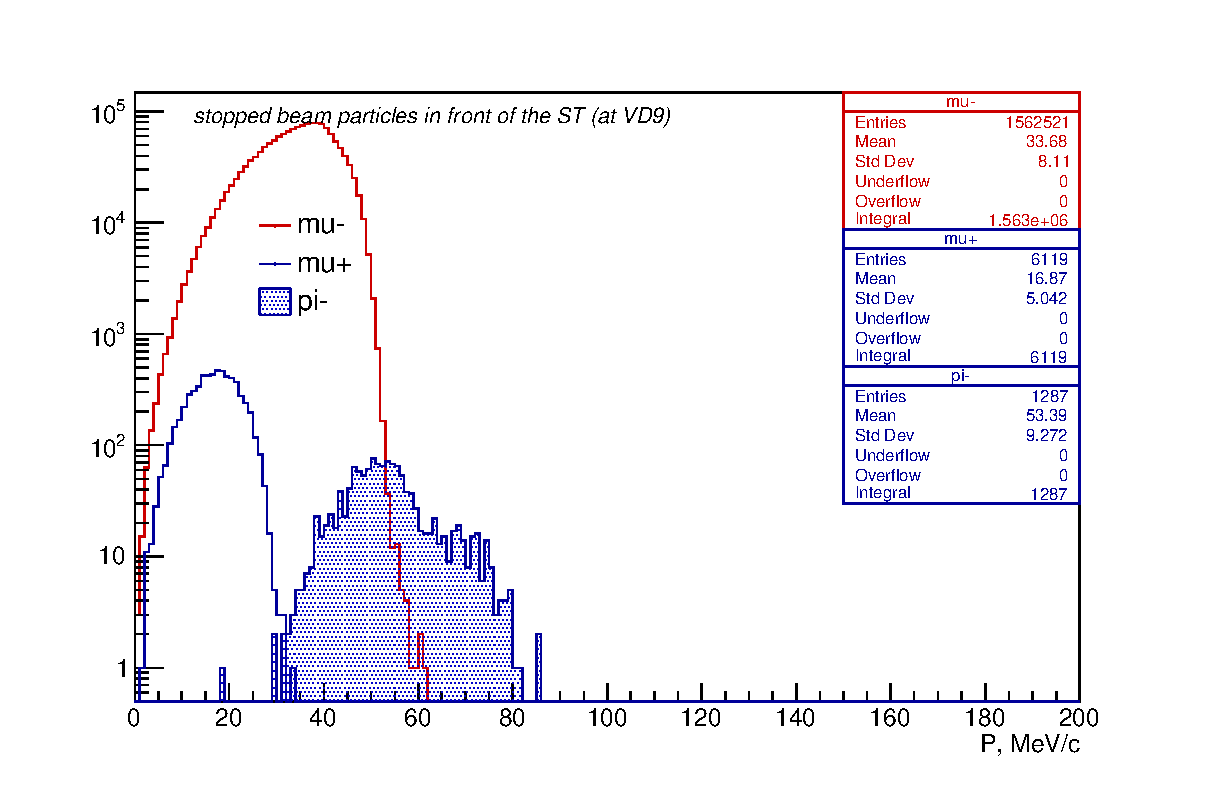
\includegraphics[width=0.6\textwidth]{figures/pdf/figure_03100_bmum0s31b0_vdet_xx09_mom}
      % }
    };
  \end{tikzpicture}
  \caption{
    \label{fig:03700_bmum0s37b0_vdet_xx09_mom}
    Left: momentum distributions of particles reaching VD9;
    Right: momentum distributions at VD9 of particles stopped in the stopping target
  }
\end{figure}

%%%%%%%%%%%%%%%%%%%%%%%%%%%%%%%%%%%%%%%%%%%%%%%%%%%%%%%%%%%%%%%%%%%%%%%%%%%%%%

\section {Beam electrons}

The red distribution in Figure \ref{fig:bmum0s16b0_momentum}(left) shows the $p ~>~ 100~\MeVc$
tail of the momentum distribution of electrons arriving at the TS31 collimator.
The blue distribution shows electrons which went through the TS31,2 collimators
and reached the TS5 collimator. Comparison of the distributions shows that for high momentum electrons
the transport efficiency is quite low, about $2\times10^{-3}$.
Figure \ref{fig:bmum0s16b0_momentum}(left) shows the corresponding timing distributions.
The tail in the timing distribution is likely due to the spread of electron production angles
in the PS - a fraction of forward produced electrons should get reflected by the PS magnetic mirror.

\begin{figure}[H]
  \hspace{-0.5in}
  \begin{tikzpicture}
    \node[anchor=south west,inner sep=0] at (0,0.) {
      % \node[shift={(0 cm,0.cm)},inner sep=0,rotate={90}] at (0,0) {}
      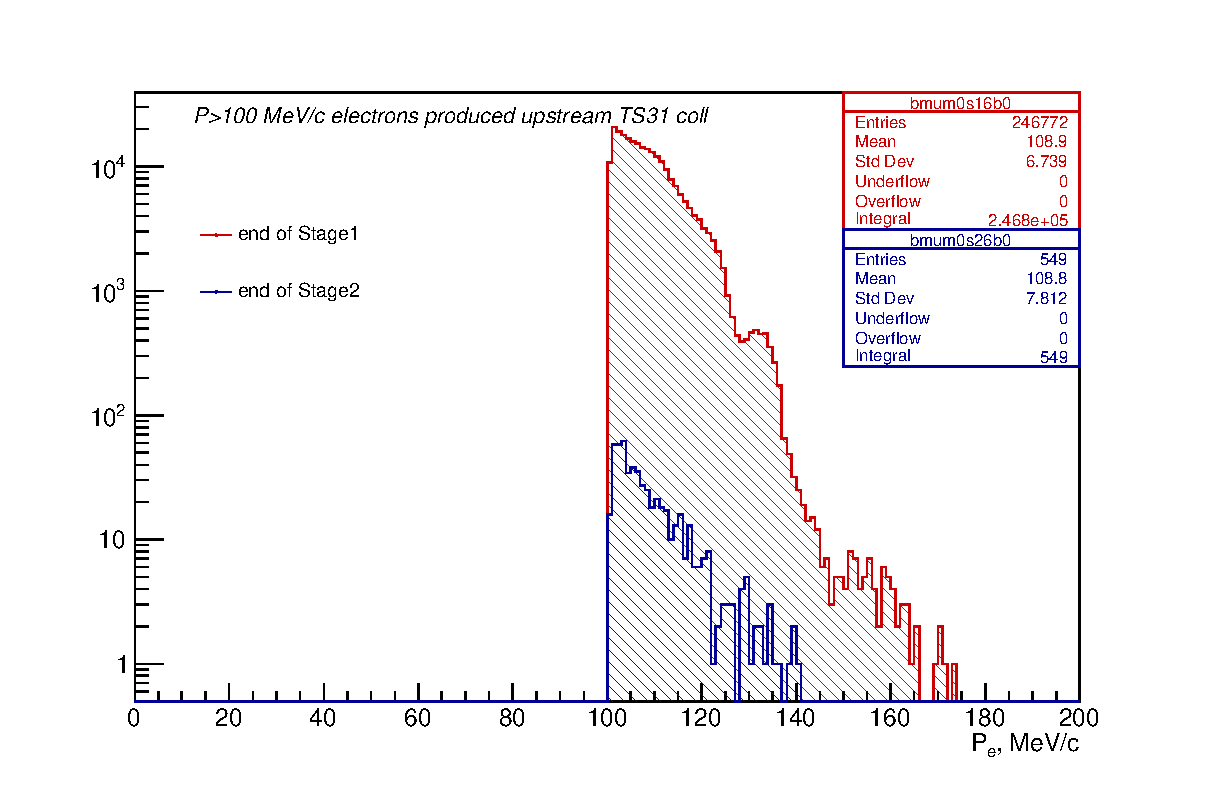
\includegraphics[width=0.6\textwidth]{figures/pdf/figure_00160_bmum0s16b0_vdet_102_mom}
    };
    \node[anchor=south west,inner sep=0] at (10., 0.) {
      % \node[shift={(0 cm,0.cm)},inner sep=0,rotate={90}] at (0,0) {}
      % \makebox[\textwidth][c] {
      \includegraphics[width=0.6\textwidth]{figures/pdf/figure_00161_bmum0s16b0_vdet_102_time}
      % }
    };
  \end{tikzpicture}
  \caption{
    \label{fig:bmum0s16b0_momentum}
    Electrons produced at Stage 1. Left: momentum distribution; Right:
    timing distribution, no beam timing smearing, just the travel times
  }
\end{figure}


To identify electrons produced in muon decays during Stage2, events which didn't have 100 \MeVc\
electrons at Stage1 are traced through Stage2 separately.

Figure \ref{fig:bmum0s26b0_momentum} overlays momentum and timing distributions in the end of Stage2
for electrons produced at Stage1 and electrons produced at Stage2. In front of TS5 collimator,
the fraction of events with electrons produced at Stage 2 is about 2\% of electrons produced
at Stage1.

\begin{figure}[H]
  \hspace{-0.5in}
  \begin{tikzpicture}
    \node[anchor=south west,inner sep=0] at (0,0.) {
      % \node[shift={(0 cm,0.cm)},inner sep=0,rotate={90}] at (0,0) {}
      % \makebox[\textwidth][c] {
      \includegraphics[width=0.6\textwidth]{figures/pdf/figure_00260_bmum0s26b0_vdet_106_mom}
      % }
    };
    \node[anchor=south west,inner sep=0] at (10., 0.) {
      % \node[shift={(0 cm,0.cm)},inner sep=0,rotate={90}] at (0,0) {}
      % \makebox[\textwidth][c] {
      \includegraphics[width=0.6\textwidth]{figures/pdf/figure_00261_bmum0s26b0_vdet_106_time}
      % }
    };
  \end{tikzpicture}
  \caption{
    \label{fig:bmum0s26b0_momentum}
    Electrons produced at Stage 2
  }
\end{figure}

%%%%%%%%%%%%%%%%%%%%%%%%%%%%%%%%%%%%%%%%%%%%%%%%%%%%%%%%%%%%%%%%%%%%%%%%%%%%%% 
\subsection {Electrons Entering the Detector Envelope}

After the beam is traced up to the at the virtual detector VD9, surviving are:
\begin{itemize}
\item
  21 events with electrons produced at Stage1 (upstream the TS31 collimator)
\item
  9 events with electrons produced at Stage2 (in between the TS31 and TS5 collimators)
\item
  11 events with electrons produced at Stage3 (inside the TS5 collimator and in the DS,
  before the stopping target)
\end{itemize}

With the aim on understanding the effect of scattering in the stopping target,
the events are re-simulated (re-sampled) $10^4$ times.
Events with electrons entering the detector envelope are left for analysis.
%
The two-dimensional distributions of cos(theta) vs momentum for those events
are shown in Figures \ref{fig_bmum0s56b0_cth_vs_mom} and \ref{fig_bmum0s59b0_cth_vs_mom}.
Effect of oversampling is clearly seen, however, as all events are simulated with
the unit weight, which reduces importance of oversampling.

\begin{figure}[h]
  \hspace{-0.5in}
  \begin{tikzpicture}
    \node[anchor=south west,inner sep=0] at (0,0.) {
      % \node[shift={(0 cm,0.cm)},inner sep=0,rotate={90}] at (0,0) {}
      % \makebox[\textwidth][c] {
      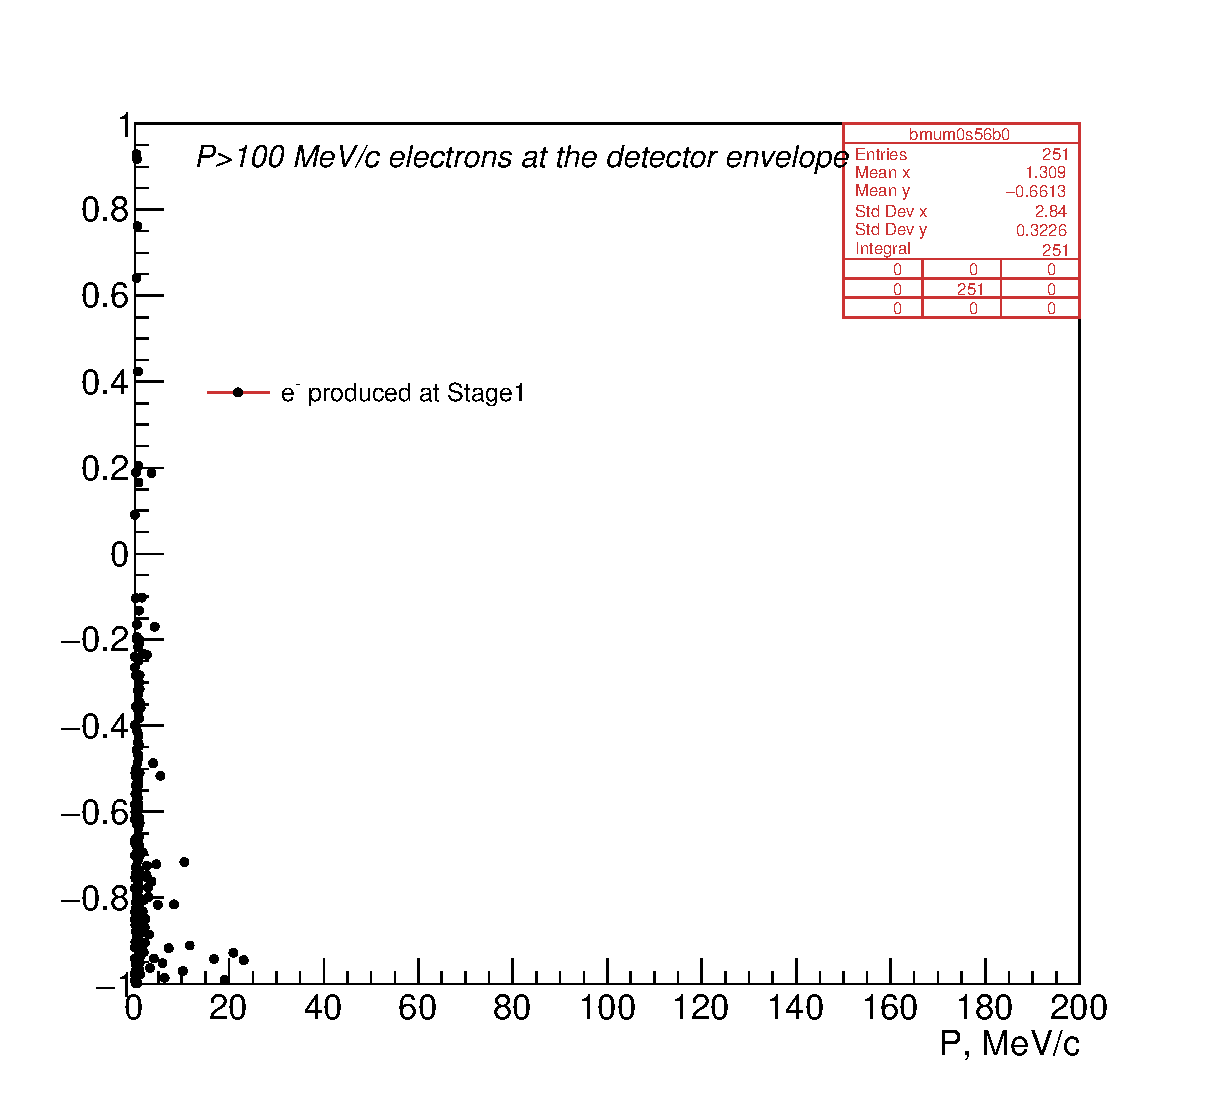
\includegraphics[width=0.55\textwidth]{figures/pdf/figure_00560_bmum0s56b0_spmc_1_cth_vs_mom_1}
      % }
    };
    \node[anchor=south west,inner sep=0] at (10,0.) {
      % \node[shift={(0 cm,0.cm)},inner sep=0,rotate={90}] at (0,0) {}
      % \makebox[\textwidth][c] {
      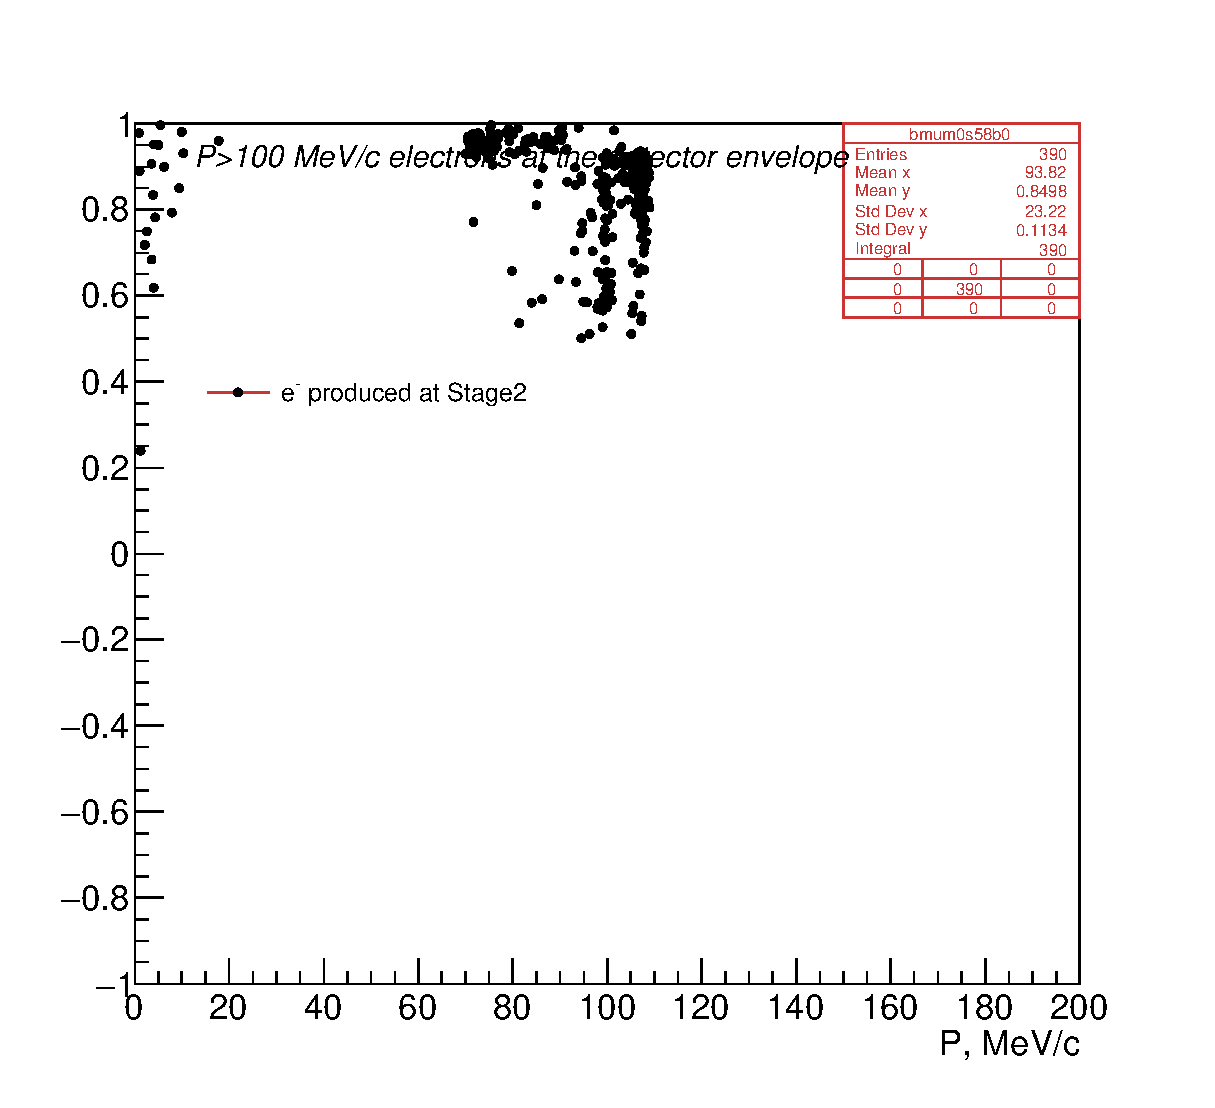
\includegraphics[width=0.55\textwidth]{figures/pdf/figure_00580_bmum0s58b0_spmc_1_cth_vs_mom_1}
      % }
    };
  \end{tikzpicture}
  \caption{
    \label{fig_bmum0s56b0_cth_vs_mom}
    Electrons produced at Stage1 and Stage2 entering the detector envelope
  }
\end{figure}
    
\begin{figure}[h]
  \hspace{-0.5in}
  \begin{tikzpicture}
    \node[anchor=south west,inner sep=0] at (0,-9.) {
      % \node[shift={(0 cm,0.cm)},inner sep=0,rotate={90}] at (0,0) {}
      % \makebox[\textwidth][c] {
      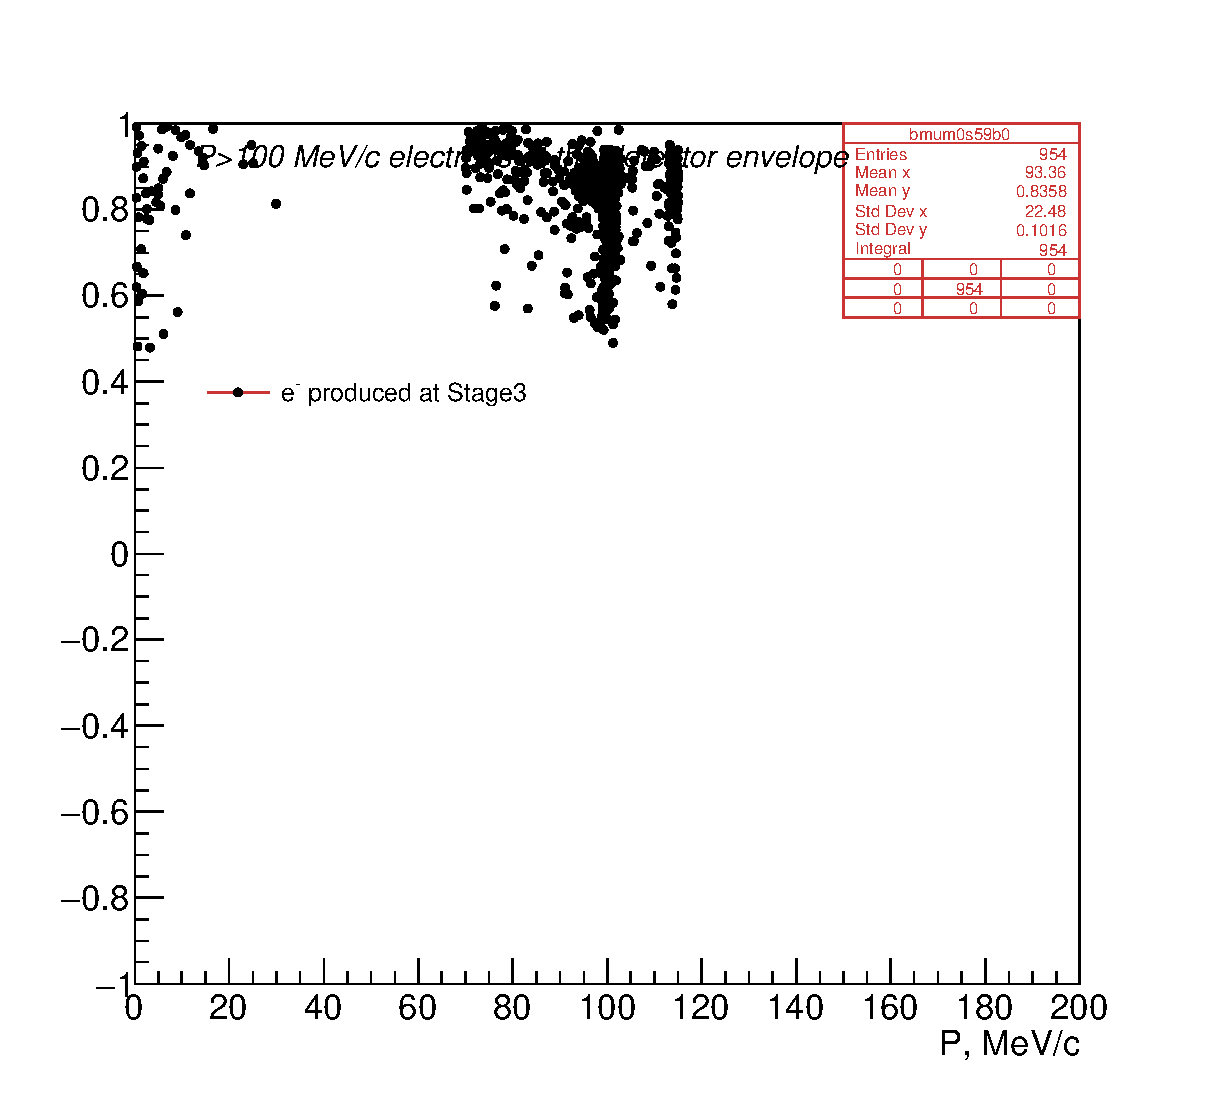
\includegraphics[width=0.55\textwidth]{figures/pdf/figure_00590_bmum0s59b0_spmc_1_cth_vs_mom_1}
      % }
    };
  \end{tikzpicture}
  \caption{
    \label{fig_bmum0s59b0_cth_vs_mom}
    Electrons produced at Stage3 and entering the detector envelope
  }
\end{figure}

Figure \ref{fig:bmum0s56b0_spmc_1_mom}(left) shows momentum distributions for electrons
entering the detector envelope with $0 < \cos \theta < 0.71$,
which gives a very loose definition of the reconstruction cuts.
After the $\cos \theta$ selection, the contribution of electron production
at Stage1 becomes negligibly small.

\begin{figure}[H]
  \hspace{-0.5in}
  \begin{tikzpicture}
    \node[anchor=south west,inner sep=0] at (0,0.) {
      % \node[shift={(0 cm,0.cm)},inner sep=0,rotate={90}] at (0,0) {}
      % \makebox[\textwidth][c] {
      \includegraphics[width=0.6\textwidth]{figures/pdf/figure_01561_bmum0s59b0_spmc_1_mom}
      % }
    };
    \node[anchor=south west,inner sep=0] at (10,0.) {
      % \node[shift={(0 cm,0.cm)},inner sep=0,rotate={90}] at (0,0) {}
      % \makebox[\textwidth][c] {
      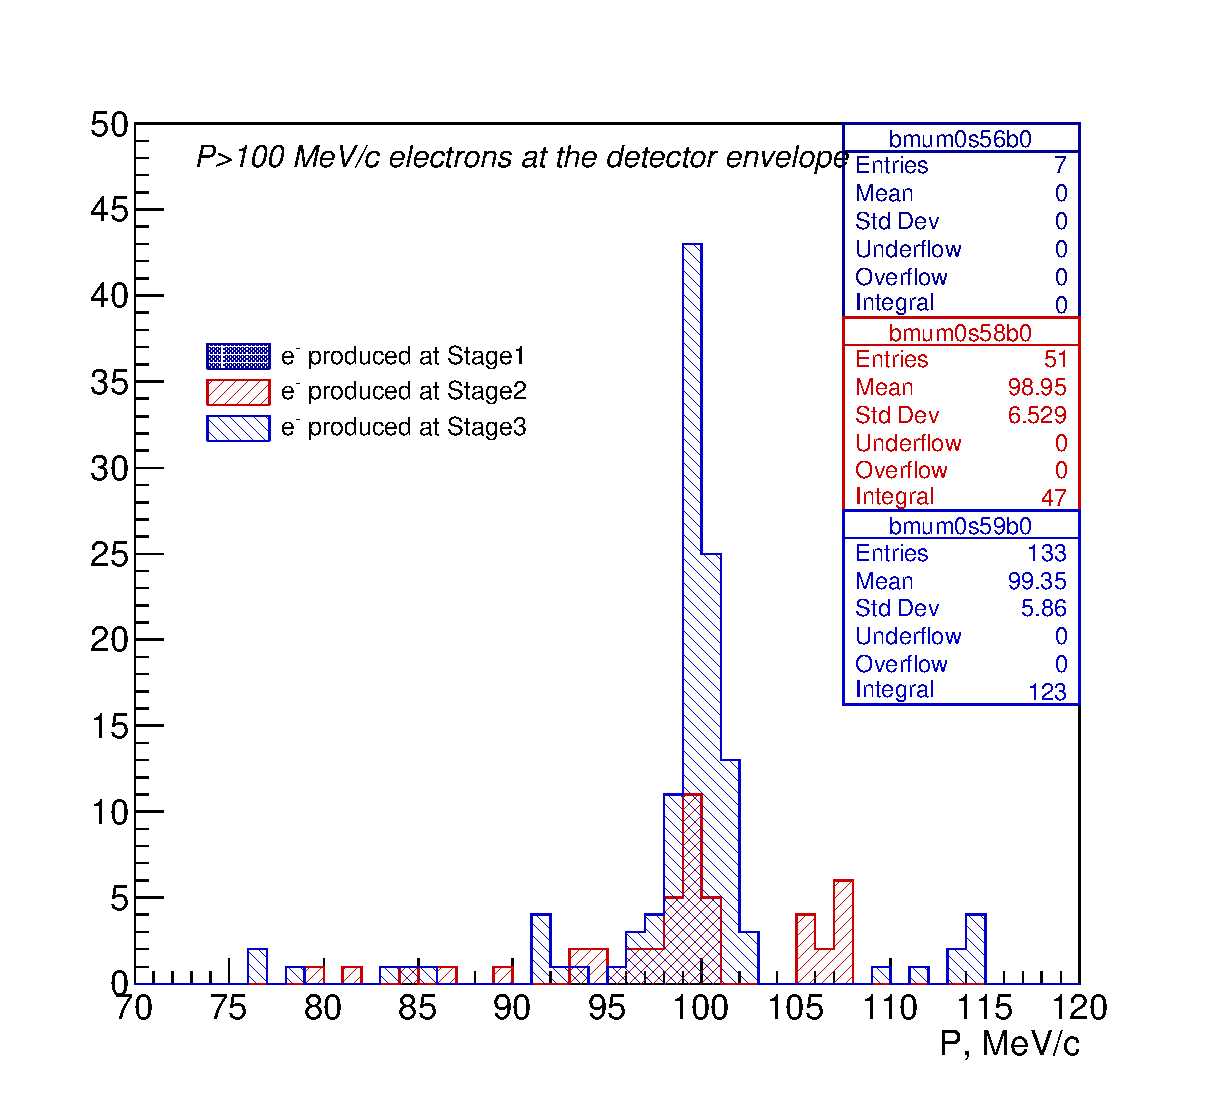
\includegraphics[width=0.6\textwidth]{figures/pdf/figure_01562_bmum0s59b0_spmc_1_mom}
      % }
    };
  \end{tikzpicture}
  \caption{
    \label{fig:bmum0s56b0_spmc_1_mom}
    Momentum distribution of electrons entering the detector envelope
    after scattering in the stopping target.
    The left and the right plots show the same events, the right plot zooms
    in on the momentum region around 100 \MeVc.
  }
\end{figure}

Figure \ref{fig:bmum0s56b0_spmc_1_mom}(right) zooms in on a momentum range of interest.
Contribution of electrons with $p ~<~ 102 ~\MeVc$ is negligible. 
Assume flat distribution between 102 and 115 MeV/c, the signal window of 1.5 \MeVc\ (instead of 1.3 \MeVc),
and the proton beam extinction of $1 \times 10^{-10}$. Normalization to the total proton flux
of $4 \times 10^{19}$ protons on target gives the expected background mean of 
$$
    N_{\rm ele} ~=~ 23/13 \times 1.5 \times 4 \times 10^{19} ({\rm N_{POT}}) \times 10^{-10}  ({\rm extinction}) / 10^{13} ({\rm statistics}) ~\simeq ~ 1 \times 10^{-3}
$$

As the number above assumes the track reconstruction efficiency for a particle entering
the tracker envelope volume to be 100\%, this number represents an upper limit on
the contribution from the electrons scattered in the stopping target.
The estimate is higher than the TDR estimate \cite{MU2E_6464_CD3_BEAM_ELECTRONS},
which didn't take into account muon decays in and downstream the TS5 collimator.
Still, it is low enough to be a source of concern.
It should be noted that the beam electron background is dominated by electrons
produced by muon decays in flight in TSd and DS, after the TS3 collimator.
This contribution is not sensitive to the vertical misalignments of the beamline, 
and, in particular, to relatively small variations of the PS magnetic field.

%%%%%%%%%%%%%%%%%%%%%%%%%%%%%%%%%%%%%%%%%%%%%%%%%%%%%%%%%%%%%%%%%%%%%%%%%%%%%%
\section {Muon decays in flight}

To produce a 100 MeV/c electron, a decaying muon has to have its momentum $p ~>~ \sim$ 72 \MeVc.
Muons with momentum $\sim 70 \MeVc$ arrive into the DS early, and the background
from muons produced by ``in-time'' protons is rejected by the timing window.
However the contribution of muons produced by the out-of-time protons needs
to be taken into account.
%
To estimate this contribution, muons traced down to VD9 are re-simulated 1000 times each,
and events with electrons entering the detector envelope volume are selected for further analysis.
%
Figure \ref{fig:bmum0sb8b0_cth_vs_mom}(left) shows the two-dimensional distribution 
of cos(theta) vs momentum for selected events.
The kinematic region of interest, shown on the plot by the hashed rectangle,
contains no events.

\begin{figure}[H]
  \hspace{-0.5in}
  \begin{tikzpicture}
    \node[anchor=south west,inner sep=0] at (0,0.) {
      % \node[shift={(0 cm,0.cm)},inner sep=0,rotate={90}] at (0,0) {}
      % \makebox[\textwidth][c] {
      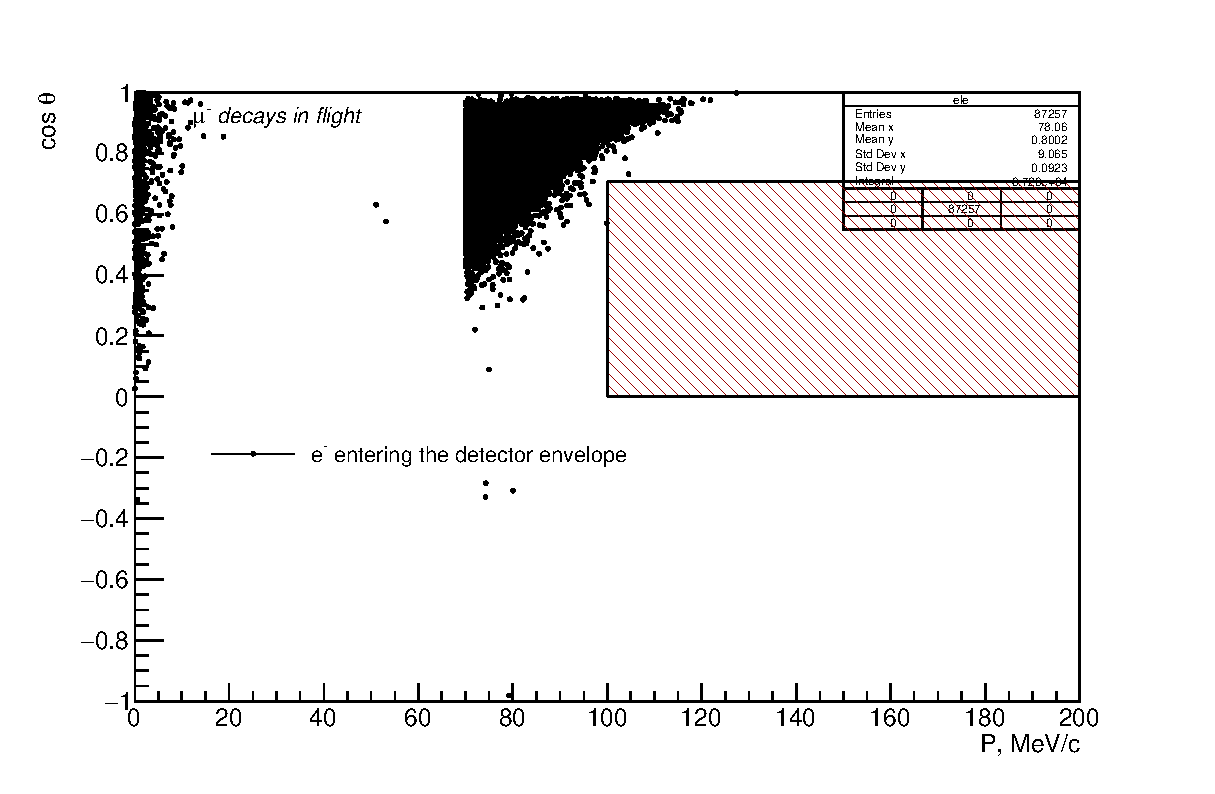
\includegraphics[width=0.5\textwidth]{figures/pdf/figure_04000_bmum0s5bb0_spmc_1_cth_vs_mom}
      % }
    };
    \node[anchor=south west,inner sep=0] at (10,0.) {
      % \node[shift={(0 cm,0.cm)},inner sep=0,rotate={90}] at (0,0) {}
      % \makebox[\textwidth][c] {
      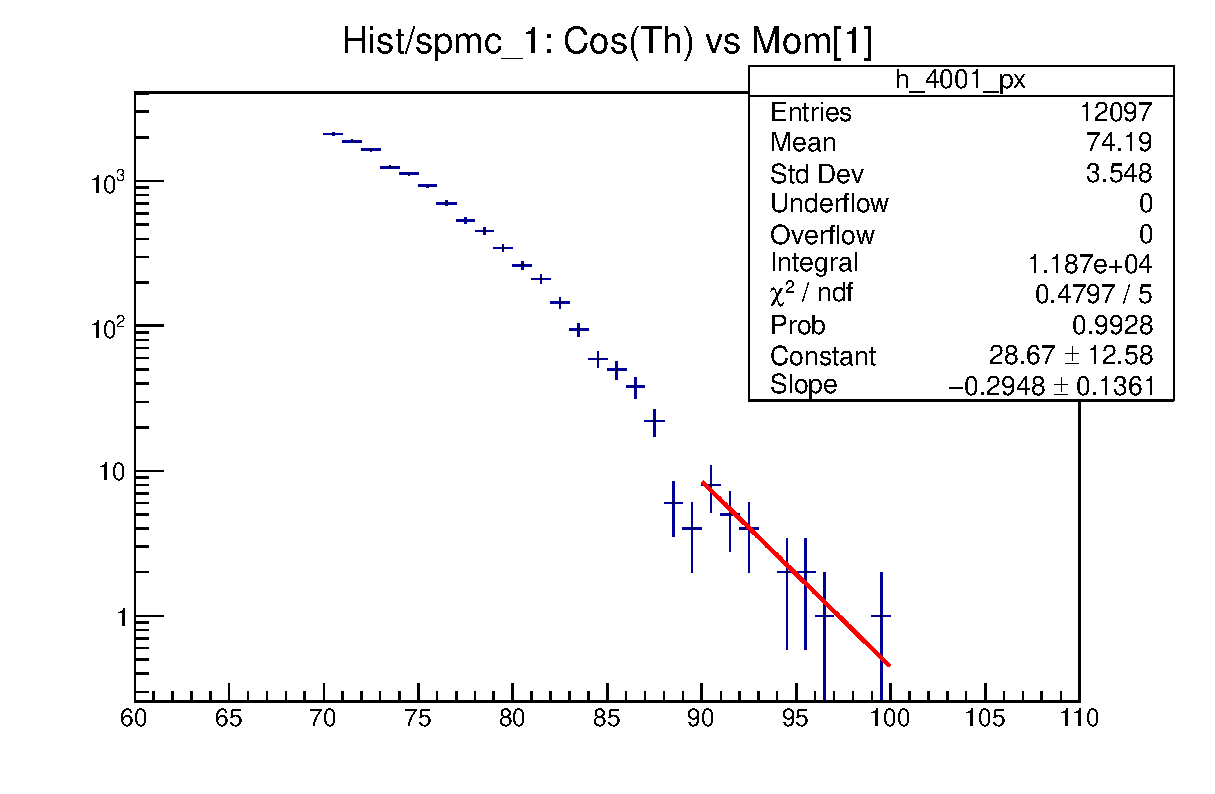
\includegraphics[width=0.5\textwidth]{figures/pdf/figure_04001_bmum0s5bb0_spmc_1_cth_vs_mom}
      % }
    };
  \end{tikzpicture}
  \caption{
    \label{fig:bmum0sb8b0_cth_vs_mom}
    Electrons from muon decays downstream VD9 entering the detector envelope
  }
\end{figure}

Figure \ref{fig:bmum0sb8b0_cth_vs_mom}(right) shows the momentum distribution
for events with cos(theta) < 0.71. Also shown is the binned log likelihood fit
of the distribution in the range 90-100 \MeVc with an exponential. 
An upper bound on the contribution from muon decays in flight is determined
by extrapolating the fit function to higher momenta, integrating it over the
region [103.5, 105.0] \MeVc\ and normalizing the integral to the total proton
beam flux expected in Run I, $4 \times 10^{19}$ POT :
\begin{equation}
  \label{eqq_001}
N_{\rm DIF} ~=~ I \times {\frac{N_{\rm POT}}{N_{\rm sim} \cdot R}}  \times f_{\rm ext}
\end{equation}
In the equation above, $I$ is the integral of the extrapolated fit function over [103.5,105.0] \MeVc.

\noindent
Using $I ~=~ 0.18$ events, $N_{\rm sim} ~=~ 10^9$ events,
the resampling factor $R ~=~ 1000$, and the beam extinction factor $f_{\rm ext} ~=~ 10^{-10}$
gives 
$$
N_{\rm DIF} ~=~ 7.2 \times 10^{-4} ~<~ 1  \times 10^{-3}
$$
  
This upper bound is about three times higher than the CD3 estimate
of \cite{MU2E_4342_MUON_DECAYS_IN_FLIGHT_TDR} - $3\times 10^{-3}$ for the proton flux $N_{POT} ~=~ 3.6\times 10^{20}$,
but still small, much smaller than the uncertainty on the cosmic background.

Compared to negative muons, the number of pions arriving to DS is suppressed
by a factor of $\sim$ 400.
We therefore expect the contribution of pion decays in DS to be small compared
to the contribution of muon decays.
%
This expectation is different from the conclusion of \cite{MU2E_4342_MUON_DECAYS_IN_FLIGHT_TDR},
where the contribution of pion decays has been estimated at a level of 30\% from muon decays.
As the branching ratio of  $B(\pi \ra e \nu) ~=~~ 1.2 \times 10^{-4}$, 
significant part of the pion contribution should come from $\pi \ra \mu \nu$ 
decays followed by $\mu \ra e \nu\nu$ decays, and $N(\pi \ra e)/N(\mu \ra e) ~\sim~ 30\%$
seems to be a conservative number
%%%%%%%%%%%%%%%%%%%%%%%%%%%%%%%%%%%%%%%%%%%%%%%%%%%%%%%%%%%%%%%%%%%%%%%%%%%%%%
\section {Muon scattering in the ST}

As shown in Figure \ref{fig:03700_bmum0s37b0_vdet_xx09_mom}, the momentum distribution
of muons arriving to DS extends above 100 \MeVc. 
Muons scattered in the stopping target, reconstructed and misidentified as electrons
contribute to the background. 
To be reconstructed in the delayed timing window, a 100 \MeVc\ muon has to be produced
by the out-of-pulse proton. Therefore, similar to the sources discussed in the previous
sections, the background from muon scattering in the stopping target is suppressed
by the proton beam extinction.

To estimate this background, muons with $p ~>~ 100 ~\MeVc$ traced up to VD9,
are resimulated $10^4$ times each and retained for analysis are events with muons
entering the detector fiducial. Momentum distribution for muons with $\cos\theta < 0.71$
is shown in Figure \ref{fig_bmum0sb8b0_crt_vs_mom}(right).
In the region $p ~>~ 100 ~\MeVc$, the momentum distribution is fit with a constant.
Normalization of the integration over the region [103.5,105] \MeVc\
to the expected Run I proton beam flux gives
\begin{equation}
   N_{\rm scattered~ \mu} ~=~ I \times {\frac{N_{\rm POT}}{N_{\rm sim} \cdot R}}  \times f_{\rm ext} \times P_{\rm misID}
\end{equation}
, where $R ~=~ 10^4$ is the resampling factos and $ P_{\rm misID} ~=~ 0.01$ is a conservative
estimate of the probability to mis-identify a reconstructed muon as an electron.
Substitution of the numbers into the equation above gives
$$
 N_{\rm scattered~ \mu} < 1 \times 10^{-5}
$$

\begin{figure}[H]
  \hspace{-0.5in}
  \begin{tikzpicture}
    \node[anchor=south west,inner sep=0] at (0,0.) {
      % \node[shift={(0 cm,0.cm)},inner sep=0,rotate={90}] at (0,0) {}
      % \makebox[\textwidth][c] {
      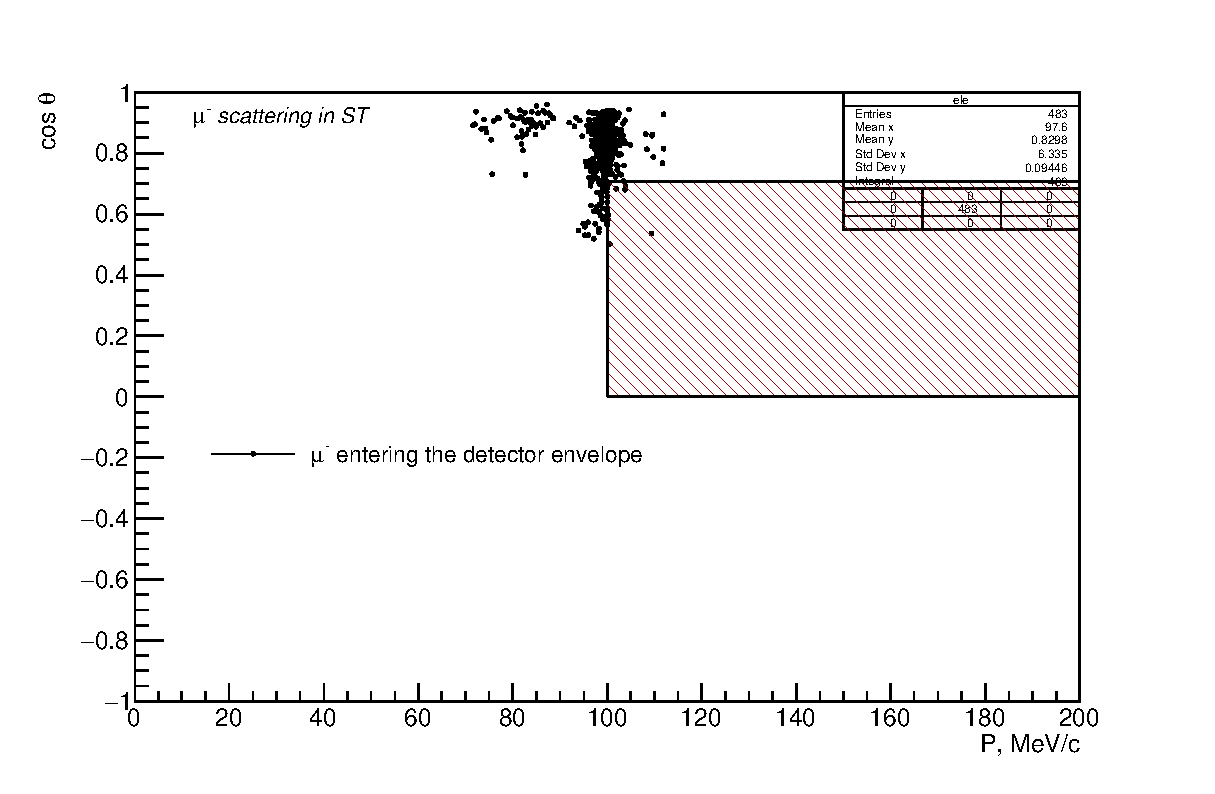
\includegraphics[width=0.5\textwidth]{figures/pdf/figure_04100_bmum0s5ab0_spmc_1_cth_vs_mom}
      % }
    };
    \node[anchor=south west,inner sep=0] at (10,0.) {
      % \node[shift={(0 cm,0.cm)},inner sep=0,rotate={90}] at (0,0) {}
      % \makebox[\textwidth][c] {
      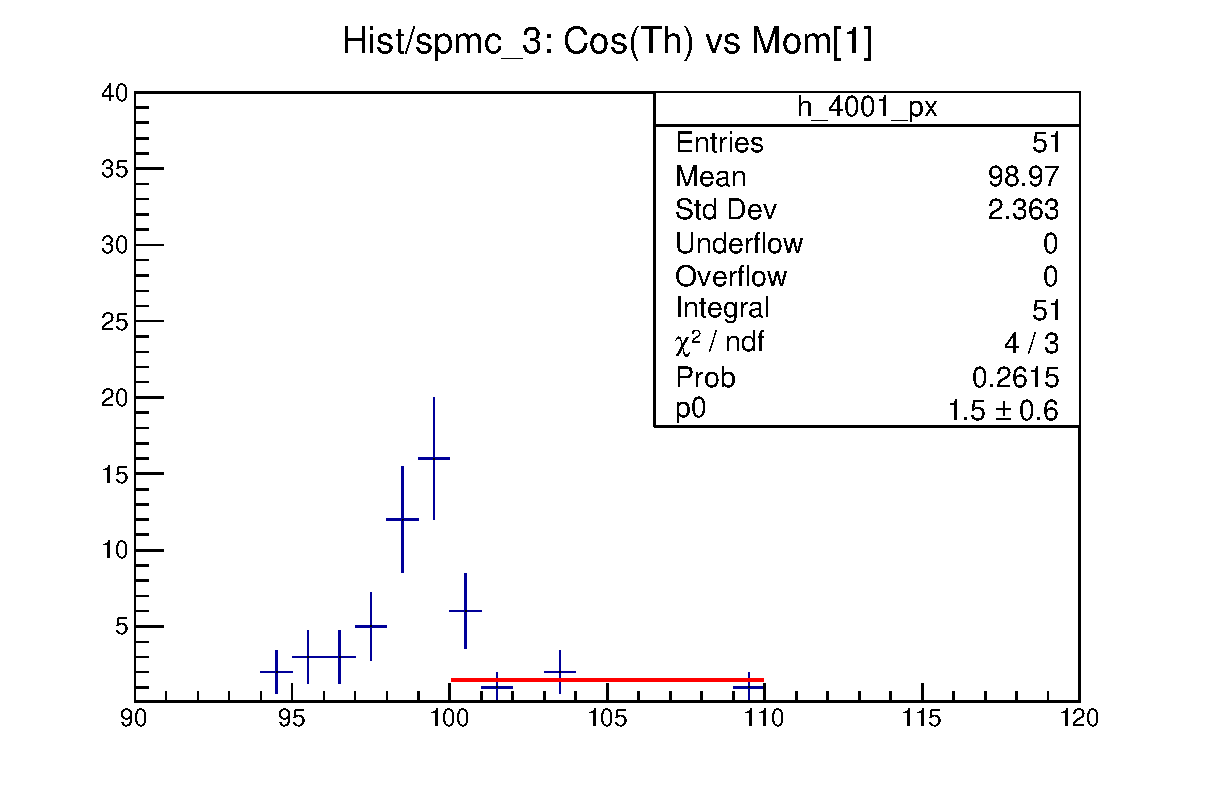
\includegraphics[width=0.5\textwidth]{figures/pdf/figure_04101_bmum0s5ab0_spmc_1_cth_vs_mom}
      % }
    };
  \end{tikzpicture}
  \caption{
    \label{fig_bmum0sb8b0_crt_vs_mom}
    Electrons from muon decays downstream VD9 entering the detector envelope
  }
\end{figure}

%%%%%%%%%%%%%%%%%%%%%%%%%%%%%%%%%%%%%%%%%%%%%%%%%%%%%%%%%%%%%%%%%%%%%%%%%%%%%%
\newpage
\section {Mu2e Timing Cartoon}

Figure \ref{fig:03160_flsh0s36b0_vdet_9_time}, in a simplified form, shows the
timing structure of the Mu2e measurement. 
At T=0 a proton pulse arrives at the production target.
In about 80 ns after that particles produced at the production target start arriving
into the DS. The total number of beam flash particles with $E > 0.1 ~MeV$ is about 20\%
from the number of protons per pulse. Most of them are low energy electrons and positrons
with $E > 10 ~MeV$. 
%
Muons are about 1\% of the total, negative pions are suppressed by an additional factor of $\sim$ 250.
%
\noindent
Optimized for Run I signal window starts at 640 ns, below which the 
An upper edge at 1650 ns avoids early background from the next proton pulse.

\begin{figure}[H]
  % \hspace{-0.6in}
  \begin{tikzpicture}
    \node[anchor=south west,inner sep=0] at (0,0.) {
      % \node[shift={(0 cm,0.cm)},inner sep=0,rotate={90}] at (0,0) {}
      \makebox[\textwidth][c] {
      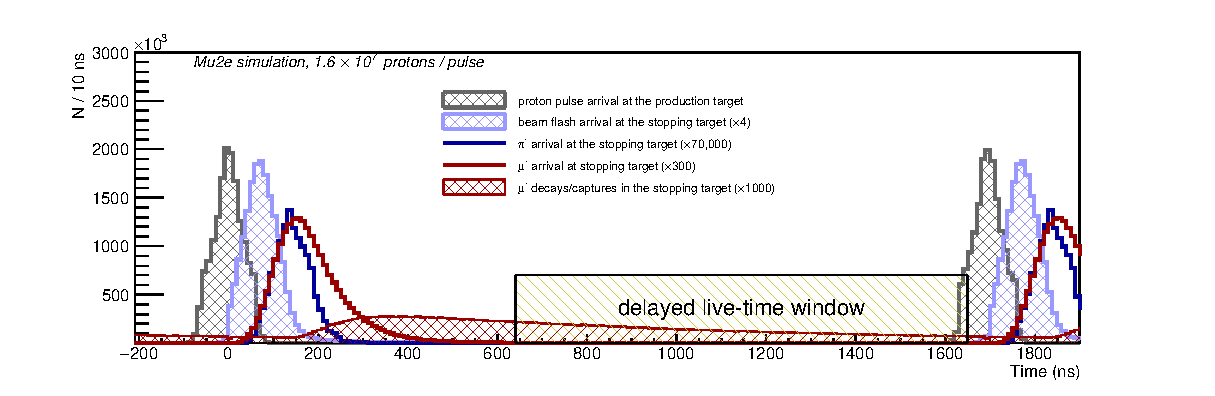
\includegraphics[width=1.2\textwidth]{figures/png/figure_03160_flsh0s36b0_vdet_9_time}
    }
    };
  \end{tikzpicture}
  \caption{
    \label{fig:03160_flsh0s36b0_vdet_9_time}
    Mu2e beam timing diagram
  }
\end{figure}



%%%%%%%%%%%%%%%%%%%%%%%%%%%%%%%%%%%%%%%%%%%%%%%%%%%%%%%%%%%%%%%%%%%%%%%%%%%%%%
\newpage
\section{Summary}
Upper bounds on the direct beam-related backgrounds are as follows:
\begin{itemize}
\item
  background from beam electrons scattered in the stopping target < $1 \times 10^{-3}$
\item
  background from muon decay in flights < $1 \times 10^{-3}$
\item
  background from beam muons scattered in the stopping target < $1 \times 10^{-5}$
\end{itemize}
%%%%%%%%%%%%%%%%%%%%%%%%%%%%%%%%%%%%%%%%%%%%%%%%%%%%%%%%%%%%%%%%%%%%%%%%%%%%%%
%
%%%%%%%%%%%%%%%%%%%%%%%%%%%%%%%%%%%%%%%%%%%%%%%%%%%%%%%%%%%%%%%%%%%%%%%%%%%%%%
\newpage
\bibliographystyle{unsrtnat}
\bibliography{local,clfv,dio,mu2e_internal_notes}

\end{document}

%%%%%%%%%%%%%%%%%%%%%%%%%%%%%%%%%%%%%%%%%%%%%%%%%%%%%%%%%%%%%%%%%%%%%%%%%%%%%%
% small font sizes: \small \footnotesize \scriptsize \tiny
% ------------------------------------------------------------------------------
% templates
% ------------------------------------------------------------------------------
% Table ~\ref{table:summary} gives summary the numbers used in this study.
%
% \hspace{-0.1in}
% \begin{table}[htbp]
%   \label{table:summary}
%   \begin{center}
%     {\renewcommand{\arraystretch}{1.0}   % change 1.0 to 1.1 to increase the spacing between the table lines
%       \begin{tabular}{|c|c|c|c|}
%         \hline
%                             & default TS geometry & misaligned TS geometry   &  Ratio(default/misaligned)    \\
%         \hline
%         $N_{POT}$            &  $4.96 \cdot 10^6$  &    $5.00 \cdot 10^6$      &   0.992   \\
%         $N_{\mu}^{TS3u}$      &  65648              &     61354                 &   1.070   \\
%         $N_{\mu}^{TS5}$       &  28517              &     27351                 &   1.043   \\
%         $N_{\mu}^{ST}$        &  8868               &      8396                 &   1.056   \\
%         $N_{\mu}^{ST}/N_{POT}$ &  $1.79 \pm 0.02$    &    $1.68 \pm 0.02$        &   $1.065 \pm 0.03$        \\
%         \hline
%       \end{tabular}
%     }
%   \end{center}
%   \caption{
%     Muons rates at different points of the Mu2e beamline and stopping muon rates for nominal and
%     misaligned TS geometries
%   }
%   % \vspace{0.5in}
% \end{table}
